\begin{savequote}
\quoteperson{They can't keep this level of graphics up for much longer!
We used to be lucky if we only got three shades of gray, let alone any 
real colours!}{Cranky Kong}
\end{savequote}

\chapter{Hardware Assisted Geometric Algebra on the GPU}

In this chapter we explore how the \emph{Graphics Processing
Units} (GPUs) in modern consumer-level graphics cards can be
used to perform Geometric Algebra computations faster than a 
typical single-core CPU.

\section{An Overview of GPU Architecture}

\begin{figure}
\centering
\includegraphics[width=0.9\textwidth]{gpu_architecture}
\caption{\label{fig:gpu_architecture}%
  A simplified block diagram of a typical GPU.}
\end{figure}

The GPU in a graphics card is not designed for general purpose 
computing. It is designed, not suprisingly, to perform the
sort of operations useful for graphics rendering. Figure
\ref{fig:gpu_architecture} shows a simplified block diagram of
a typical GPU.

In a traditional fixed-function GPU the CPU uploads, over the AGP
bus, a set of vertices, texture maps and some state information. The
state includes projection matrices, view matrices, clipping planes, 
lighting models, etc. The vertex list and texture maps (if present) 
are then stored in some on-card memory.

On the card there exists a number of rendering pipelines, each of which
can be run in parallel to increase throughput. The pipeline consists
of a \emph{vertex shader} which fetches triplets of vertices from
the vertex memory, transforms them using the current projection and 
view matrices, performs any clipping and sends them to the rasterizer.

The rasteriser takes triplets of screen co-ordinate vertices, forms
a triangle from them and outputs a set of pixel positions which form
render the triangle along with depth information and interpolated texture
co-ordinates. 

The fragment shader takes these pixel positions and, using the texture maps
stored in texture memory along with appropriate state information calculates
the colour of the pixel after all lighting, etc. is performed. The shaded pixel
is then sent to the screen.

In reality the rendering stage is split at the rasterizer allowing for differing
numbers of vertex and fragment shaders but for the purposes of GPU programming
one can view the shaders as being within the same pipeline.

In modern programmable GPUs both the vertex and fragment shaders are fully 
programmable allowing different per-vertex and per-pixel transformation
and shading that is allowed in the traditional fixed-function pipeline.

Each shader is, in effect, an efficient vector processor and, on modern 
graphics cards, there are a number working in parallel. To perform
general purpose computation on the GPU we must find ways of modifying our
algorithms to fit this model.

\section{GPU Programming Methods}

\subsection{DirectX shader language}

Microsoft's DirectX\cite{GPU:DirectX} is a graphics programming API for
Windows and, to some extent, the Microsoft XBox gaming platform. As part of
the API it specifies a generic shading language\cite{GPU:DirectXShadingLanguage}
which abstracts the vertex and fragment shaders. Each version of DirectX
specifies a minimum set shader capabilities which \emph{must} be supported by a 
card claiming compatibility with that level of the API. Consequently a shader written in
DirectX's shading language is portable across all cards which support that level
of the API. A disadvantage of DirectX is that it doesn't expose any functionaility
beyond the specified minimum and it is not portable across operating systems.

\subsection{OpenGL shader language}

OpenGL\cite{GPU:OpenGLSpec} is a cross-platform C-based graphics API. 
It is the \emph{de facto} standard API for non-Windows platforms and
is well supported on Windows platforms by both ATI and nVidia, the dominant
vendor at the time of writing. 

The OpenGL 2.0 specification\cite{GPU:OpenGL2Overview} proposed by 3DLabs
includes a hardware agnostic shading language\cite{GPU:OpenGLShadingLanguage}
known as \emph{GL Shading Language} (GLSL) which provides a similar level
of functionality to that exposed in DirectX. 

Currently few hardware vendors support OpenGL 2.0 --- at the time of writing
nVidia was the only mainstream vendor to provide support in their
consumer-level hardware\cite{nvidia:7664relnotes}.

OpenGL 1.4 and below provide support for programmable shaders via a set of per-vendor
extensions. Unfortunately these requires progamming the GPU in a variety of
assembly languages and vary between different GPUs.

\subsection{The Cg toolkit from nVidia}

Both the OpenGL and DirectX shading languages have a number of disadvantages
from the point of view of research. The OpenGL shading language, whilst being
high-level and convenient to program in, is not widely available. The
DirectX toolkit porvides only a `lowest common denomitator' shading language,
it is not particularly high-level and is, for all intents and purposes, limited
to the Microsoft Windows operating systems. 

An attempt to bridge these gaps is the Cg toolkit\cite{nvidia:cgtoolkit} from nVidia.
It provides a high-level C-like shading language which may be compiled at run-time or
ahead of time into either DirectX shading language or the myrriad of OpenGL extensions
which exist for accessing the programmable shaders. 

Along with these advantages is the `future-proof' nature of Cg. The core Cg language
is easily extended via so-called `profiles'. These either restrict the language to
correspond to the capabilities of particular GPUs or add more features to expose
new GPU abilities. As an example in figure \ref{fig:gpu_architecture} it was implied
that the vertex shader cannot access the texture-map memory. This was true
of older cards but the latest generation of nVidia cards can
access texture maps from within the vertex shader\cite{nvidia:sm3unleashed}. Adding this
capability to Cg was simply a case of releasing a new profile where texture-map related
parts of the language were now available from within both shaders. Older shaders
would still work however and the presence of this capability could be queried
at run-time.

Because of these advantages it was decided to use Cg as the basis for the GPU
computing research. None of the techniques described below require it as they
can all be re-structured to use alternate APIs.

\section{Mesh deformation}

In this section we shall give an example of a vertex shader that uses GA to
perform mesh deformation.

FIXME: Medium-length review of mesh deformation.

\subsection{Method}

We shall now present a GA-based mesh deformation scheme. In this scheme we start with
an existing mesh and set of key rotors, $\left\{ R_1, R_2, \cdots, R_k \right\}$,
which we wish to use to deform the mesh. Our scheme seeks to find some automatic
method of representing each point on the mesh as some function of the key
rotors; changing the key rotors will then lead to a deformation of the mesh. Desirable
properties include smoothness, small changes in the rotors lead to small changes
in the mesh, and intuitivity, changes in the rotors should produce changes
in the mesh which a user, ignorant of the method, would expect.

\begin{figure}
\centering
\includegraphics[width=0.8\textwidth]{assignment_scheme}
\caption{\label{fig:assignment_scheme}Representing a point, $P_i$, on a mesh as
a rotor, $R_i$, and displacement, $p_i$, given a set of key rotors, 
  $\left\{R_1, R_2\right\}$.}
\end{figure}

Our assignment scheme is illustrated in figure \ref{fig:assignment_scheme}.
Firstly we form a set of generators, $\left\{B_1, B_2, \cdots, B_k\right\}$,
such that
\[
\left\{ R_1, R_2, \cdots, R_k \right\} \equiv \left\{\exp(B_1), \exp(B_2),
        \cdots, \exp(B_k)\right\}.
\]
We also find the image of the origin, $O_k = R_k\bar{n}\tilde{R}_k$, for 
each key-rotor. For each point-representaion on the mesh, $P_i$, we find the Euclidean
distance from it to the image of the origin in each key-rotor,
\[
\label{eqn:dki}
d_{k,i} = \sqrt{-2O_k \cdot P_i}.
\]
We then form a rotor, $R_i$, for each point on the mesh as a weighted sum of the
key-rotors,
\[
R_i = \exp\left(\frac{\sum^{k}_1 w_i(d_{k,i}) B_i}{\sum^{k}_1 w_i(d_{k,i})}\right)
\]
where $w_i(d)$ is a function which defines the relative weights of each rotor depending
on its proximity to the mesh point. One might choose a relatively simple weight function
\[
w_i(d) = \frac{1}{d + \epsilon}
\]
where $\epsilon$ is a small value to avoid a singularity when the key-rotor and mesh
intersect. If our implementation we wished to have key-rotors with varying degrees of influence.
This was accomplished by using a Gaussian weight function,
\[
w_i(d) = \exp\left(-\frac{d^2}{\sigma_i^2}\right)
\]
with $\sigma_i$ giving the radius of influence of a particular key-rotor.

Finally we find a point, $p_i$, which is transformed by $R_i$ to coincide
with $P_i$,
\[
(R_i p_i \tilde{R}_i) \cdot P_i = 0
\]
which may be found by simply applying the reversal of $R_i$ to $P_i$
\[
p_i = \tilde{R}_i P_i R_i.
\]
The point $P_i$ is now stored in memory as a set of $d_{k,i}$ for each
key-rotor and the point $p_i$.

Our deformation procedure is now simple. Given a new set of key-rotors,
$\left\{ R'_1, R'_2, \cdots, R'_k \right\}$, and a corresponding set of
generators, $\left\{B'_1, B'_2, \cdots, B'_k\right\}$, we can form the deformed
mesh point $P'_i$ given the previously calculated $d_{k,i}$ and $p_i$ as
\begin{align}
R'_i &= 
\exp\left(\frac{\sum^{k}_1 w_i(d_{k,i}) B'_i}{\sum^{k}_1 w_i(d_{k,i})}\right) \label{eqn:summation} \\
P'_i &= R'_i p_i \tilde{R}'_i.
\end{align}

\subsection{GPU-based implementation}

Since the GPU distinguishes between global state and per-vertex information we
must decide what information needs to be given to the GPU and how. In our mesh
deformation example we need the key-rotors which are part of the global state
and, for each mesh point, the vector $p_i$ and set of distances $d_{k,i}$.

In OpenGL each vertex has at least a three-dimensional position vector associated 
with it and may have a normal vector. In addition there are a number of 
texture co-ordinates which may be associated with each vertex. In our implmentation
the values of $w(d_{k,i})$ will be stored into the texture co-ordinates. The weight
function is pre-computed to save time.

\begin{figure}[p]
\centering
\scalebox{0.8}{
\begin{minipage}{\textwidth}
\singlespacing
\lstinputlisting[language=c]{vertex_shader.cg}
\end{minipage}}
\caption{\label{fig:meshshader}The vertex shader used to perform GA-based mesh
deformation.}
\end{figure}

Figure \ref{fig:meshshader} gives the vertex shader used to perform mesh deformation in
this example. Line 2 includes the standard set of rotor manipulation functions which
will be described below. For the moment it is sufficient to note that generators are
stored as a pair of 3-vectors, giving 6 components in all, and rotors are stored as a
pair of 4-vectors, giving 8 components.

The generators associated with the key rotors are passed in the state array {\tt generators[][]}
and are constant for a particular scene. Lines 32 to 39 perform the summation in 
equation \ref{eqn:summation} and line 41 uses the function {\tt exp\_generator()} to 
form $R'_i$. Line 42 applies $R'_i$ to the point $p_i$ and the remainder of the shader
is bolierplate code to project into screen-space and perform a simple lighting calculation.

\begin{fancyalg}
\begin{algorithmic}[1]
\REQUIRE{$P_i$, the null-vector representation of mesh vertex $i$.}
\REQUIRE{$\mathcal{B} \equiv \{B_1, B_2, \cdots, B_k, \cdots \}$,
  the set of key-rotor generators.}
\STATE $w_{\mathrm{sum}} := 0$
\FOR{$k := 1$ to $n(\mathcal{B})$}
\STATE $R := \exp(B_k)$
\STATE $O := R\bar{n}\tilde{R}$
\STATE $w_k := w(\sqrt{-2 O \cdot P})$
\STATE $w_{\mathrm{sum}} := w_{\mathrm{sum}} + w_k$
\ENDFOR
\FOR{$k := 1$ to $n(\mathcal{B})$}
\STATE $w_k := \frac{w_k}{w_{\mathrm{sum}}}$
\ENDFOR
\STATE $p := \tilde{R}P_iR$
\STATE glMultiTexCoord2f(GL\_TEXTURE0, $w_1$, $w_2$);
\STATE glMultiTexCoord2f(GL\_TEXTURE1, $w_3$, $w_4$); 
\STATE glMultiTexCoord2f(GL\_TEXTURE2, $w_5$, $w_6$);
\STATE glMultiTexCoord2f(GL\_TEXTURE3, $w_7$, $w_8$);
\STATE glVertex($p$);
\end{algorithmic}
\caption{\label{alg:meshpoint}Algorithm for computing $w(d_{k,i})$ and $p_i$ for 
  each mesh point and storing them in the texture co-ordinates and vertex position.
  In this case there are eight key-rotors.}
\end{fancyalg}

The algorithm and OpenGL code required to compute the rotor wieghts and offset-vector
$p_i$ for each mesh vertex is shown in algorithm \ref{alg:meshpoint}. Note that this
need only be performed once-per vertex at initialisation.

In the actual implementation \emph{display lists} were utilised. A display list 
is an OpenGL technique for uploading a set of OpenGL calls to the graphics card
and executing them again with one call. Since the vertices and texture co-ordinates
generated by algorithm \ref{alg:meshpoint} don't change once calculated each mesh could
be processed once and sent to the graphics card as a display list.

Using a display list meant that the deformation now became extremely efficient in
terms of CPU usage. For each frame all that needed to be done by the CPU was update the
state variables holding the key-rotor generators and ask for the display list to be drawn.
Using such a technique resulted in the Unix \emph{top} utility reporting 0\% CPU utilisation,
i.e. below the resolution it measures to.

\subsection{Quality of the deformation}

\begin{figure}[p]
\centering
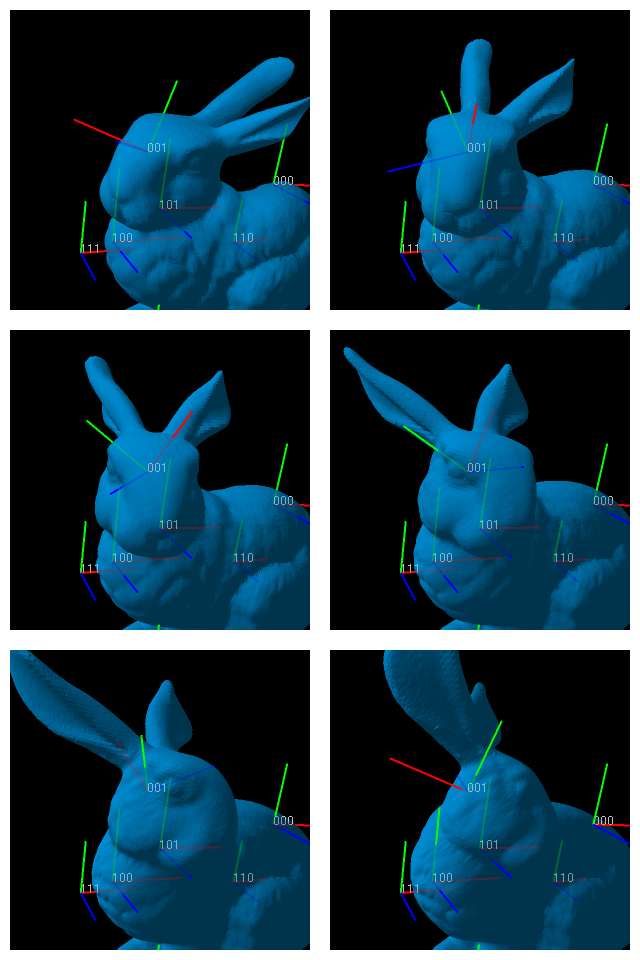
\includegraphics[height=0.8\textheight]{mesh_example}
\caption{\label{fig:meshexample}An example of animating a rabbit's head using key-rotors and an automatically
  assigned mesh.}
\end{figure}

The quality of a mesh deformation technique is ultimately subjective. A simple example is shown
in figure \ref{fig:meshexample}. In this example there were eight key rotors labelled `000' to
`111' in binary. The rotors were moved to positions within a rabbit model and appropriate
weighting and offset-vectors were assigned using algorithm \ref{alg:meshpoint}. The `001' rotor,
which was positioned within the rabbit's head, was then moved and the results are shown.
The movement is smooth, natural and intuitive.

\begin{figure}[p]
\centering
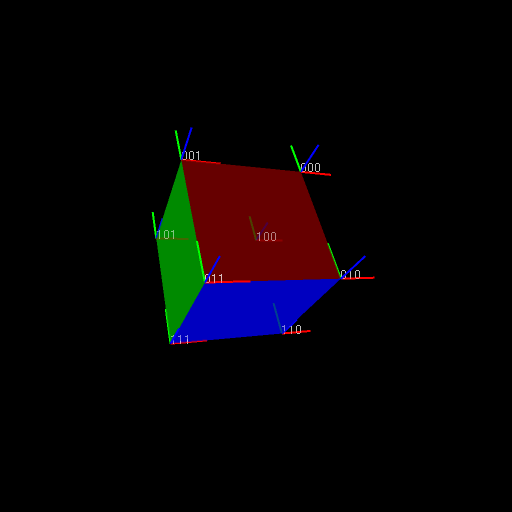
\includegraphics[height=0.37\textheight]{cube_before} \\
\noindent (a) \\ \rule{0pt}{\parskip} \\
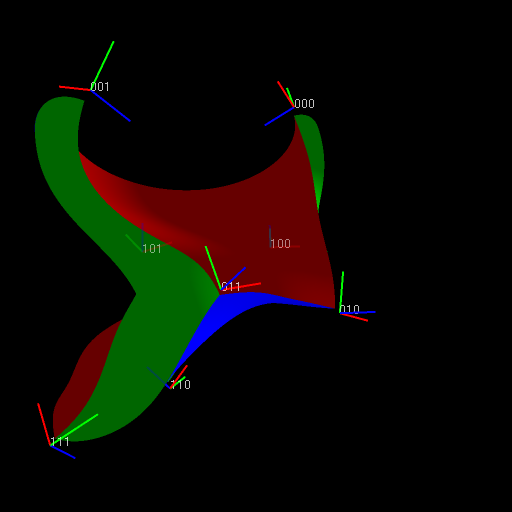
\includegraphics[height=0.37\textheight]{cube_after} \\
\noindent (b) 
\caption{\label{fig:cubeexample}An example of mesh deformation acting on a unit cube.
  (a) Initial key-rotors and automatically assigned mesh. 
  (b) Deformed mesh after movement of key-rotors.} 
\end{figure}

\section{Cloth simulation}

In this section we shall give an example of a fragment shader which is used to
perform a simple cloth simulation.
